% !TeX root = surprises.tex

\selectlanguage{hebrew}


\chapter{אפשר להסתפק במחוגה}\label{c.compass}

%%%%%%%%%%%%%%%%%%%%%%%%%%%%%%%%%%%%%%%%%%%%%%%%%%%%%%%%%%%%%%%

בשנת
$1797$
\L{Lorenzo Mascheroni}
הוכיח שכל בניה גיאומטרית באמצעות סרגל ומחוגה ניתנת לבניה עם מחוגה בלבד. במאה העשרים התגלה שהמשפט הוכח בשנת
$1672$
על ידי
\L{Georg Mohr}.
המשפט נקרא היום משפט
\L{Mohr-Mascheroni}.
לאחר שנסביר בסעיף%
~\ref{s.compass-what}
מה המשמעות של בניית ללא מחוגה, נביא את ההוכחה בשלבים, תחילה עם ארבע בניות עזרה: שיקוף של נקודה (סעיף%
~\ref{s.reflection}),
בניית מעגל עם רדיוס נתון (סעיף%

~\ref{s.circle}),
חיבור וחיסור של קטעי קו (סעיף%
~\ref{s.add-subtract})
ובניית קטע קו כיחס בין קטעים אחרים (סעיף%
~\ref{s.three}).
סעיף%
~\ref{s.two-lines}
מראה איך למצוא את החיתוך בין שני קווים וסעיף%
~\ref{s.line-circle}
מראה איך למצוא את החיתוך בין קו ומעגל.

%%%%%%%%%%%%%%%%%%%%%%%%%%%%%%%%%%%%%%%%%%%%%%%%%%%%%%%%%%%%%%%

\section{מהי בנייה רק עם מחוגה}\label{s.compass-what}

מה המשמעות של בניה גיאומטרית באמצעות  מחוגה בלבד ללא סרגל? איור%
~\ref{f.compass-equi}
מראה את הבניה הרגילה של משולש שווה צלעות עם סרגל ומחוגה. איך אפשר לבנות משולש ללא קטעי הקווים
$\overline{AB},\overline{AC},\overline{BC}$?
למעשה, אין כל צורך
\textbf{לראות}
את הקווים. קו מוגדר על ידי שתי נקודות, ומספיק שבנו את הנקודות 
$A,B,C$
 כדי לקבל בניה שקולה לבניה עם סרגל (איור%
~\ref{f.compass-equi-only}).

\begin{figure}[htb]
\begin{center}
\begin{subfigure}{.4\textwidth}
\begin{tikzpicture}[scale=0.6]
\coordinate (A) at (0,0);
\coordinate (B) at (4,0);
\path (A) node[below left] {$A$} -- (B) node[below right] {$B$};
\fill (A) circle[radius=2pt];
\fill (B) circle[radius=2pt];
\draw[name path=larc] (A) ++(-10:4cm) arc (-10:80:4cm);
\draw[name path=rarc] (B) ++(-170:4cm) arc (-170:-260:4cm);
\path [name intersections={of=larc and rarc,by={t}}];
\fill (t) node[above right,xshift=-2pt,yshift=3pt] {$C$} circle[radius=2pt];
\end{tikzpicture}
\caption{בניית משולש שווה צלעות עם סרגל ומחוגה}\label{f.compass-equi}
\end{subfigure}
\hspace{3em}
\begin{subfigure}{.4\textwidth}
\begin{tikzpicture}
\coordinate (A) at (0,0);
\coordinate (B) at (4,0);
\draw (A) node[below left] {$A$} -- (B) node[below right] {$B$};
\fill (A) circle[radius=2pt];
\fill (B) circle[radius=2pt];
\draw[name path=larc] (A) ++(-10:4cm) arc (-10:80:4cm);
\draw[name path=rarc] (B) ++(-170:4cm) arc (-170:-260:4cm);
\path [name intersections={of=larc and rarc,by={t}}];
\fill (t) node[above right,xshift=-2pt,yshift=3pt] {$C$} circle[radius=2pt];
\draw (A) -- (t);
\draw (B) -- (t);
\end{tikzpicture}
\caption{בניית משולש שווה צלעות רק עם מחוגה}\label{f.compass-equi-only}
\end{subfigure}
\end{center}
\end{figure}
באיורים נצייר בכל זאת קווים, אולם הקווים משמשים אך ורק להבנת הבניה ולהוכחת נכונותה. חשוב להשתכנע שהבניה עצמה משתמשת רק במחוגה.


כל צעד בבניה באמצעות סרגל ומחוגה הוא אחת משלושת הפעולות הבאות:
\begin{itemize}
\item
מציאת נקודת החיתוך של שני קווים.
\item
מציאת נקודות החיתוך בין קו ומעגל.
\item
מציאת נקודות החיתוך בין שני מעגלים.
\end{itemize}
ברור שניתן לבצע את הפעולה השלישית רק עם מחוגה. עלינו להראות שעבור שתי הפעולות הראשונות ניתן למצוא בניה שקולה שמשתמשת רק במחוגה.


נשתמש בסימונים:
\begin{itemize}
\item $C(O,A)$: 
המעגל שמרכזו
$O$
העובר דרך הנקודה
$A$.
\item $C(O,r)$:
המעגל שמרכזו
$O$
עם רדיוס
$r$.
\item $C(O,\overline{AB})$:
המעגל שמרכזו
$O$
עם רדיוס שהוא אורך קטע הקו
$\overline{AB}$.
\end{itemize}

%%%%%%%%%%%%%%%%%%%%%%%%%%%%%%%%%%%%%%%%%%%%%%%%%%%%%%%%%%%%%%%

\section{שיקוף נקודה}\label{s.reflection}

\begin{definition}
הנקודה
$C'$
היא
\textbf{%
שיקוף%
}
של הנקודה
$C$
מסביב לקטע הקו
$\overline{AB}$,
אם 
$\overline{AB}$
)או הקו המכיל אותו( הוא האנך האמצעי של
$\overline{CC'}$.
\end{definition}
\begin{theorem}\label{thm.reflection}
נתון קטע קו
$\overline{AB}$
ונקודה 
$C$
שלא נמצאת על
$\overline{AB}$.
ניתן לבנות נקודה 
$C'$
שהיא השיקוף של
$C$
מסביב ל-%
$\overline{AB}$.
\end{theorem}

\begin{proof}
בנו מעגל שמרכזו
$A$
העובר דרך
$C$
ומעגל שמרכזו
$B$
העובר דרך
$C$.
נקודות החיתוך של שני המעגלים הן הנקודה
$C$
והנקודה
$C'$
שהיא השיקוף של
$C$
(איור%
~\ref{f.compass-reflection}).
\begin{figure}[htb]
\begin{center}
\begin{tikzpicture}[scale=.75]
\coordinate (A) at (0,0);
\coordinate (B) at (4,0);
\coordinate (C) at (2.5,1.5);
\draw[thick,name path=ab] ($(B)!2!(A)$) -- ($(A)!2!(B)$);
\fill (A) node[above left] {$A$} circle[radius=2pt];
\fill (B) node[above right] {$B$} circle[radius=2pt];
\fill (C) node[above,yshift=4pt] {$C$} circle[radius=2pt];
\node[draw,circle through=(C),name path=ac] at (A) {};
\node[draw,circle through=(C),name path=bc] at (B) {};
\path [name intersections={of=ac and bc,by={x1,Cp}}];
\fill (Cp) node[below,yshift=-4pt] {$C'$} circle[radius=2pt];
\draw (C) -- (Cp);
\draw[rotate=90] ($(C)!.5!(Cp)$) rectangle +(8pt,8pt);
\draw[thick] (A) -- (C);
\draw[thick] (B) -- (C);
\draw[thick] (A) -- (Cp);
\draw[thick] (B) -- (Cp);
\end{tikzpicture}
\caption{בניית שיקוף}\label{f.compass-reflection}
\end{center}
\end{figure}

$\triangle ABC\cong\triangle ABC'$
חופפים לפי צלע-צלע-צלע:
$\overline{AC},\overline{AC'}$
הם רדיוסים של אותו מעגל כמו גם
$\overline{BC},\overline{BC'}$,
ו-%
$\overline{AB}$
הוא צלע משותף. מכאן ש-%
$\angle CAB = \angle C'AB$,
ולכן
$\overline{AB}$
הוא חוצה הזווית של
$\angle CAC'$.
$\triangle CAC'$
שווה-שוקיים, וחוצה הזווית
$\overline{AB}$
הוא גם האנך האמצעי של בסיס המשולש
$\overline{CC'}$.
מכאן ש-%
$C'$
היא השיקוף של
$C$
מסביב ל-%
$\overline{AB}$.
\end{proof}

%%%%%%%%%%%%%%%%%%%%%%%%%%%%%%%%%%%%%%%%%%%%%%%%%%%%%%%%%%%%%%%

\section{בניית מעגל עם רדיוס נתון}\label{s.circle}

\begin{theorem}\label{thm.radius}
נתונות הנקודות
$A,B,C$.
ניתן לבנות את המעגל
$c(A,\overline{BC})$.
%
%שמרכזו 
%$A$
%עם רדיוס שווה לאורך של 
%$\overline{BC}$.
\end{theorem}



בנו את המעגלים 
$c(A,B)$, $c(B,A)$
וסמנו את נקודות החיתוך
$X,Y$
(איור%
~\ref{f.compass-circle1}).
\begin{figure}[htb]
\begin{center}
\begin{tikzpicture}[scale=.5]
\coordinate (A) at (0,1.5);
\coordinate (B) at (0,-1.5);
\coordinate (C) at (1.5,-3);
\coordinate (Cp) at (1.5,3);
\vertex{A};
\vertex{B};
\vertex{C};
\node[above] at (A) {$A$};
\node[below] at (B) {$B$};
\node[below] at (C) {$C$};
\node[draw,circle through=(B),name path=ab] at (A) {};
\node[draw,circle through=(A),name path=ba] at (B) {};
\path [name intersections={of=ab and ba,by={Y,X}}];
\node[above right,xshift=4pt] at (X) {$X$};
\node[above left,xshift=-4pt] at (Y) {$Y$};
\draw[dashed] ($(X)!2!(Y)$) -- ($(Y)!2!(X)$);
\coordinate (Cp) at (1.5,3);
\vertex{Cp};
\node[above,yshift=2pt] at (Cp) {$C'$};
\draw (A) -- (B);
\draw (C) -- (Cp);
\draw (Y) -- (A) -- (X) -- (B) -- cycle;
\end{tikzpicture}
\end{center}
\caption{בניית מעגל עם רדיוס נתון (1)}\label{f.compass-circle1}
\end{figure}
%
%\begin{figure}[htb][htb]
%\begin{center}
%\begin{tikzpicture}[scale=.5]
%\coordinate (A) at (0,1.5);
%\coordinate (B) at (0,-1.5);
%\coordinate (C) at (1.5,-3);
%\coordinate (Cp) at (1.5,3);
%\fill (A) node[above] {$A$} circle[radius=3pt];
%\fill (B) node[below] {$B$} circle[radius=3pt];
%\fill (C) node[below] {$C$} circle[radius=3pt];
%%\fill (Cp) node[above] {$C'$} circle[radius=3pt];
%\node[draw,circle through=(B),name path=ab] at (A) {};
%\node[draw,circle through=(A),name path=ba] at (B) {};
%\path [name intersections={of=ab and ba,by={Y,X}}];
%\fill (X) node[above right,xshift=4pt] {$X$} circle[radius=3pt];
%\fill (Y) node[above left,xshift=-4pt] {$Y$} circle[radius=3pt];
%\draw[thick,dashed] ($(X)!2!(Y)$) -- ($(Y)!2!(X)$);
%%\draw[thick,dashed] (C) -- (Cp);
%\end{tikzpicture}
%\caption{}\label{}
%\end{center}
%\end{figure}
לפי משפט%
~\ref{thm.reflection}
בנו את
$C'$,
השיקוף של
$C$
מסביב לקו
$\overline{XY}$
(איור%
~\ref{f.compass-circle3}).

\begin{figure}[htb]
\begin{center}
\begin{tikzpicture}[scale=.6]
\coordinate (A) at (0,1.5);
\coordinate (B) at (0,-1.5);
\coordinate (C) at (1.5,-3);
\coordinate (Cp) at (1.5,3);
\node[above,yshift=2pt] at (A) {$A$};
\node[below,yshift=-2pt] at (B) {$B$};
\node[below,yshift=-2pt] at (C) {$C$};
\node[above,xshift=1pt,yshift=2pt] at (Cp) {$C'$};
\node[circle through=(B),name path=ab] at (A) {};
\node[circle through=(A),name path=ba] at (B) {};
\path [name intersections={of=ab and ba,by={Y,X}}];
\node[above right,xshift=4pt] at (X) {$X$};
\node[above left,xshift=-4pt] at (Y) {$Y$};
%\node[draw,circle through=(C)] at (Y) {};
\draw[dashed] ($(X)!1.8!(Y)$) -- ($(Y)!1.8!(X)$);
\path[name path=xy] (X) -- (Y);
\node[draw,thick,circle through=(Cp)] at (A) {};
\draw (A) -- (Cp);
\draw (B) -- (C);
\draw[name path=abline] (A) -- (B);
\draw[name path=ccp] (C) -- (Cp);
\path[name intersections={of=xy and abline,by={D}}];
\path[name intersections={of=xy and ccp,by={E}}];
\node[above left] at (D) {$D$};
\node[below right,xshift=-3pt] at  (E) {$E$};
\draw (D) -- (Cp);
\draw (D) -- (C);
\draw (D) rectangle +(9pt,9pt);
\draw (E) rectangle +(9pt,9pt);
\vertex{Y};
\vertex{A};
\vertex{X};
\end{tikzpicture}
\end{center}
\caption{בניית מעגל עם רדיוס נתון (2)}\label{f.compass-circle3}
\end{figure}
%
%\begin{figure}[htb]
%\begin{center}
%\begin{tikzpicture}[scale=.45]
%\coordinate (A) at (0,1.5);
%\coordinate (B) at (0,-1.5);
%\coordinate (C) at (1.5,-3);
%\coordinate (Cp) at (1.5,3);
%\fill (A) node[right] {$A$} circle[radius=3pt];
%\fill (B) node[right] {$B$} circle[radius=3pt];
%\fill (C) node[below,yshift=-2pt] {$C$} circle[radius=3pt];
%\fill (Cp) node[above,xshift=2pt,yshift=2pt] {$C'$} circle[radius=3pt];
%\node[circle through=(B),name path=ab] at (A) {};
%\node[circle through=(A),name path=ba] at (B) {};
%\path [name intersections={of=ab and ba,by={Y,X}}];
%\fill (X) node[above right,xshift=4pt] {$X$} circle[radius=3pt];
%\fill (Y) node[above left,xshift=-4pt] {$Y$} circle[radius=3pt];
%\node[draw,circle through=(C)] at (X) {};
%\node[draw,circle through=(C)] at (Y) {};
%\draw[thick,dashed] ($(X)!2.3!(Y)$) -- ($(Y)!2!(X)$);
%%\draw (X) -- (Y) -- (C) -- (X) -- (Cp) -- (Y);
%\draw[thick,dashed] (C) -- (Cp);
%\end{tikzpicture}
%\caption{}\label{}
%\end{center}
%\end{figure}

המעגל
$c(A,C')$
הוא המעגל המבוקש.

%\begin{center}
%\begin{tikzpicture}[scale=.5]
%\coordinate (A) at (0,1.5);
%\coordinate (B) at (0,-1.5);
%\coordinate (C) at (1.5,-3);
%\coordinate (Cp) at (1.5,3);
%\fill (A) node[above,yshift=2pt] {$A$} circle[radius=3pt];
%\fill (B) node[below,yshift=-2pt] {$B$} circle[radius=3pt];
%\fill (C) node[below,yshift=-2pt] {$C$} circle[radius=3pt];
%\fill (Cp) node[above,yshift=2pt] {$C'$} circle[radius=3pt];
%\node[circle through=(B),name path=ab] at (A) {};
%\node[circle through=(A),name path=ba] at (B) {};
%\path [name intersections={of=ab and ba,by={Y,X}}];
%\fill (X) node[above right,xshift=4pt] {$X$} circle[radius=3pt];
%\fill (Y) node[above left,xshift=-4pt] {$Y$} circle[radius=3pt];
%\node[circle through=(C)] at (X) {};
%\node[draw,circle through=(C)] at (Y) {};
%\draw[thick,dashed] ($(X)!2.3!(Y)$) -- ($(Y)!2!(X)$);
%\path[name path=xy] (X) -- (Y);
%\node[draw,thick,circle through=(Cp)] at (A) {};
%\draw[very thick] (A) -- (Cp);
%\draw[very thick] (B) -- (C);
%\draw[very thick,name path=abline] (A) -- (B);
%\draw[very thick,name path=ccp] (C) -- (Cp);
%\path [name intersections={of=xy and abline,by={D}}];
%\path [name intersections={of=xy and ccp,by={E}}];
%\fill (D) node[above left] {$D$} circle[radius=3pt];
%\fill (E) node[below right] {$E$} circle[radius=3pt];
%\draw[thick,dashed] (D) -- (Cp);
%\draw[thick,dashed] (D) -- (C);
%\end{tikzpicture}
%\end{center}

\begin{proof}
הנקודה
$A$
היא השיקוף של 
$B$
סביב 
$\overline{XY}$
)כי
$\triangle YAX\cong \triangle YBX$(, ו-%
$C'$
היא השיקוף של 
$C$
סביב
$\overline{XY}$.
לפי ההגדרה, 
$\overline{XY}$
הוא האנך האמצעי לקטעי הקו 
$\overline{AB},\overline{CC}'$,
ולכן
$\overline{C'E}=\overline{EC}$,
$\overline{AD}=\overline{DB}$,
ו-%
$\angle DEC=\angle DEC'=90^\circ$.
מכאן ש-%
$\triangle DEC\cong\triangle DEC'$
לפי צלע-זווית-צלע.
$\overline{DC}=\overline{DC'}$
ו-%
$\angle ADC'=\angle BDC$
הן זוויות משלימות ל-%
$\angle EDC', \angle EDC$.
$\triangle ADC'\cong\triangle BDC$
לפי צלע-זווית-צלע,
כך ש-%
$\overline{AC'}=\overline{BC}$.
\end{proof}

%%%%%%%%%%%%%%%%%%%%%%%%%%%%%%%%%%%%%%%%%%%%%%%%%%%%%%%%%%%%%%%

\section{חיבור וחיסור קטעי קו}\label{s.add-subtract}

\begin{theorem}\label{thm.add-subtract-mm}
נתון קטע קו
$\overline{PQ}$
באורך
$a$
וקטע קו
$\overline{RS}$
באורך
$b$.
ניתן לבנות קטע קו
%$\overline{QT},\overline{QU}$
%כך ש-%
$\overline{PUQT}$
כאשר האורך של
$\overline{PU}$
הוא
$a-b$
והאורך של
$\overline{PT}$
הוא
$a+b$
(איור%
~\ref{f.compass-add1}).
\end{theorem}

\begin{figure}[htb]
\begin{center}
\begin{tikzpicture}[scale=.8]
\coordinate (P) at (0,0);
\coordinate (Q) at (5,0);
\coordinate (T) at (3,0);
\coordinate (U) at (7,0);
\vertex{P};
\vertex{Q};
\vertex{U};
\vertex{T};
\draw (P) -- (Q);
\node[above] at (P) {$P$};
\node[above left] at (Q) {$Q$};
\node[above left] at (U) {$U$};
\node[above right] at (T) {$T$};
\draw (5,0) -- (8,0);
\coordinate (R) at (9,-1);
\coordinate (S) at ($(9,-1) + (20:2cm)$);
\vertex{R};
\vertex{S};
\draw (R) node[above] {$R$} -- node[below right] {$b$} (S) node[above] {$S$};
\draw[<->] (0,-.5) -- node[fill=white] {$a$} (5,-.5);
\draw[<->] (0,-1) -- node[fill=white] {$a-b$} (3,-1);
\draw[<->] (0,-1.5) -- node[fill=white] {$a+b$} (7,-1.5);
\end{tikzpicture}
\end{center}
\caption{חיבור וחיסור של קטעי קו}\label{f.compass-add1}
\end{figure}

%\begin{center}
%
%%\vspace*{-2ex}
%\begin{tikzpicture}[scale=.85]
%\draw (0,0) -- (5,0);
%\fill (0,0) node[above] {$P$} circle[radius=1.5pt];
%\fill (5,0) node[above left] {$Q$} circle[radius=1.5pt];
%\fill (3,0) node[above left] {$U$} circle[radius=1.5pt];
%\fill (7,0) node[above right] {$T$} circle[radius=1.5pt];
%\draw[thick,dashed] (5,0) -- (8,0);
%\draw (5,0) circle[radius=2cm];
%\draw[thick,dashed] (5,0) -- node[left] {$b$} ++(60:2cm);
%\draw (9,-1) node[above] {$R$} -- node[below right] {$b$} ++(20:2cm) node[above] {$S$};
%\fill (9,-1) circle[radius=1.5pt];
%\fill (9,-1) ++(20:2cm) circle[radius=1.5pt];
%\draw[<->] (0,-.5) -- node[fill=white] {$a$} (5,-.5);
%\draw[<->] (0,-1) -- node[fill=white] {$a-b$} (3,-1);
%\draw[<->] (0,-1.5) -- node[fill=white] {$a+b$} (7,-1.5);
%\end{tikzpicture}
%\end{center}

\begin{theorem}
ניתן לבנות טרפז שווה-שוקיים.
\end{theorem}
\begin{proof}
בחרו
$H$,
נקודה כלשהי על
$c(Q,b)$,
ובנו את
$H'$,
השיקוף שלה סביב
$\overline{PQ}$.
סמנו ב-%
$h$
האורך של
$\overline{HH'}$
(איור%
~\ref{f.compass-isoceles-trap1}).

\begin{figure}[htb]
\begin{center}
\begin{tikzpicture}[scale=.55]
\coordinate (Q) at (0,0);
\coordinate (P) at (-6.8,0);
\coordinate (B) at (-3,-2);
\draw[thick] ($(Q)!1.3!(P)$) -- node[above,near start] {$a$} ($(P)!2.3!(Q)$);
\fill (Q) node[above left] {$Q$} circle[radius=2pt];
\fill (P) node[above] {$P$} circle[radius=2pt];
\fill (B) circle[radius=2pt];
\node[draw,circle through=(B),name path=qb] at (Q) {};
\draw[thick] (Q) -- node[left,xshift=-1pt,yshift=2pt] {$b$} (B);
\path[name path=qh] (Q) -- (-40:5cm);
\path[name path=qhp] (Q) -- (40:5cm);
\path [name intersections={of=qb and qh,by={H}}];
\path [name intersections={of=qb and qhp,by={Hp}}];
\fill[below right] (H) node[right,xshift=2pt] {$H$} circle[radius=2pt];
\fill[above right] (Hp) node[right,xshift=2pt] {$H'$} circle[radius=2pt];
\draw[thick] (H) -- node[below left,yshift=-2pt] {$h$} (Hp);
\end{tikzpicture}
\caption{בניית טרפז שווה-שוקיים (1)}\label{f.compass-isoceles-trap1}
\end{center}
\end{figure}
בנו את המעגלים
$c(Q,h)$, $c(H,b)$.
$K$
היא נקודת חיתוך בין המעגלים,
ן-%
$K'$
היא השיקוף של
$K$
מסביב ל-%
$\overline{PQ}$
(איור%
~\ref{f.compass-isoceles-trap2}).

\begin{figure}[htb]
\begin{center}
\begin{tikzpicture}[scale=.5]
\coordinate (Q) at (0,0);
\coordinate (P) at (-6.8,0);
\coordinate (B) at (-3,-2);
\draw ($(Q)!1.3!(P)$) -- ($(P)!2.3!(Q)$);
\vertex{Q};
\vertex{P};
\node[above right,xshift=7pt] at (Q) {$Q$};
\node[above] at (P) {$P$};
\node[draw,circle through=(B),name path=qb] at (Q) {};
\draw (Q) -- node[left,xshift=-1pt,yshift=2pt] {$b$} (B);
\path[name path=qh] (Q) -- (-40:5cm);
\path[name path=qhp] (Q) -- (40:5cm);
\path [name intersections={of=qb and qh,by={Hp}}];
\path [name intersections={of=qb and qhp,by={H}}];
\node[right,xshift=2pt] at (H) {$H$};
\node[right,xshift=2pt] at (Hp) {$H'$};
\draw (H) -- node[below left,yshift=-3pt] {$h$} (Hp);
\vertex{H};
\coordinate (Qp) at (H|-Q);
\draw (Qp) rectangle +(10pt,10pt);
\node[above left] at (Qp) {$Q'$};
\draw[name path=circleqh] (Q) let
  \p1 = ($ (H) - (Hp) $),
  \n2 = {veclen(\x1,\y1)}
in
  circle (\n2)
  (Q) edge node[below] {$h$} +(140:\n2) ++(140:\n2) coordinate (q);
\draw[name path=circlehb] (H) let
  \p1 = ($ (Q) - (B) $),
  \n2 = {veclen(\x1,\y1)}
in
  circle (\n2)
  (H) edge node[below,near end] {$b$} +(50:\n2) ++(50:\n2)  coordinate (h);
\path [name intersections={of=circleqh and circlehb,by={K}}];
\node[above left] at (K) {$K$};
\draw let
  \p1 = ($ (K) - (Q) $)
in
  coordinate (Kp) at (\x1,-\y1);
\node[below left] at (Kp) {$K'$};
\draw (K) -- (Kp);
\draw (Q) rectangle +(10pt,10pt);
\draw[dashed] (K) -- node[right,yshift=1pt] {$b$} (H) -- (Q);
\draw[dashed] (Kp) -- (Hp) -- (Q);
\end{tikzpicture}
\end{center}
\caption{בניית טרפז שווה-שוקיים (2)}\label{f.compass-isoceles-trap2}
\end{figure}

$\overline{PQ}$
הוא האנך האמצעי של
$\overline{HH'}$
ו-%
$\overline{KK'}$,
לכן
$\overline{HH'}\|\overline{KK'}$. 
$\overline{KH} = \overline{K'H'} = b$
כי
$K$
נמצאת על
$c(H,b)$.
$K',H'$
הן שיקופים של
$K,H$,
ולכן 
$KHH'K'$
הוא טרפז שווה-שוקיים עם בסיסים
$\overline{KK'} = 2h$, $\overline{HH'}=h$
(איור%
~\ref{f.compass-isoceles-trap3}).
סמנו ב-%
$d$
את אורך האלכסונים
$\overline{K'H}=\overline{KH'}$.
\end{proof}


\begin{figure}[htb]
\begin{center}
\begin{tikzpicture}[scale=.5]
\coordinate (Q) at (0,0);
\coordinate (P) at (-6.8,0);
\coordinate (B) at (-3,-2);
\draw[dashed] ($(Q)!1.3!(P)$) -- ($(P)!2.3!(Q)$);
\node[above left] at (Q) {$Q$};
\node[above] at (P) {$P$};
\vertex{P};
\vertex{Q};
\node[draw,circle through=(B),name path=qb] at (Q) {};
\path[name path=qh] (Q) -- (-40:5cm);
\path[name path=qhp] (Q) -- (40:5cm);
\path [name intersections={of=qb and qh,by={Hp}}];
\path [name intersections={of=qb and qhp,by={H}}];
\node[right,xshift=2pt] at (H) {$H$};
\node[right,xshift=2pt] at (Hp) {$H'$};
\draw (H) -- node[below right,yshift=-2pt] {$h$} (Hp);
\path[name path=circleqh] (Q) let
  \p1 = ($ (H) - (Hp) $)
in
  circle ({veclen(\x1,\y1)});
\path[name path=circlehb] (H) let
  \p1 = ($ (Q) - (B) $)
in
  circle ({veclen(\x1,\y1)});
\path [name intersections={of=circleqh and circlehb,by={K,k2}}];
\node[above left] at (K) {$K$};
\draw (Q) -- node[left] {$h$} (K);
\draw (H) -- node[right,xshift=4pt] {$b$} (K);
\draw let
  \p1 = ($ (K) - (Q) $)
in
  coordinate (Kp) at (\x1,-\y1);
\node[below left] at (Kp) {$K'$};
\draw (Q) -- node[left] {$h$} (Kp) -- node[right,xshift=2pt,yshift=-2pt] {$b$} (Hp);
\draw (K) -- node[above right] {$d$} (Hp);
\draw (Kp) -- node[left] {$d$} (H);
\end{tikzpicture}
\end{center}
\caption{בניית טרפז שווה-שוקיים (3)}\label{f.compass-isoceles-trap3}
\end{figure}

%\begin{center}
%
%\begin{tikzpicture}[scale=.5]
%\coordinate (Q) at (0,0);
%\coordinate (P) at (-6.8,0);
%\coordinate (B) at (-3,-2);
%\draw[thick,dashed] ($(Q)!1.3!(P)$) -- ($(P)!2.3!(Q)$);
%\fill (Q) node[above left] {$Q$} circle[radius=3pt];
%\fill (P) node[above] {$P$} circle[radius=3pt];
%%\fill (B) circle[radius=3pt];
%\node[draw,circle through=(B),name path=qb] at (Q) {};
%%\draw[thick,dashed] (Q) -- node[left,xshift=-1pt,yshift=2pt] {$b$} (B);
%\path[name path=qh] (Q) -- (-40:5cm);
%\path[name path=qhp] (Q) -- (40:5cm);
%\path [name intersections={of=qb and qh,by={Hp}}];
%\path [name intersections={of=qb and qhp,by={H}}];
%\fill (H) node[right,xshift=2pt] {$H$} circle[radius=3pt];
%\fill (Hp) node[right,xshift=2pt] {$H'$} circle[radius=3pt];
%\draw (H) -- node[below right,yshift=-2pt] {$h$} (Hp);
%\path[name path=circleqh] (Q) let
%  \p1 = ($ (H) - (Hp) $)
%in
%  circle ({veclen(\x1,\y1)});
%\path[name path=circlehb] (H) let
%  \p1 = ($ (Q) - (B) $)
%in
%  circle ({veclen(\x1,\y1)});
%\path [name intersections={of=circleqh and circlehb,by={K,k2}}];
%\fill (K) node[above left] {$K$} circle[radius=3pt];
%\draw (Q) -- node[left] {$h$} (K);
%\draw (H) -- node[right,xshift=4pt] {$b$} (K);
%\draw let
%  \p1 = ($ (K) - (Q) $)
%in
%  coordinate (Kp) at (\x1,-\y1);
%\fill (Kp) node[below left] {$K'$} circle[radius=3pt];
%\draw (Q) -- node[left] {$h$} (Kp) -- node[right,xshift=2pt,yshift=-2pt] {$b$} (Hp);
%\draw (K) -- node[above right] {$d$} (Hp);
%\draw (Kp) -- node[left] {$d$} (H);
%\end{tikzpicture}\label{p.ptolemy}
%\end{center}
\begin{theorem}
ניתן לחסום טרפז שווה-שוקיים במעגל.
\end{theorem}
\begin{proof}
מייד ממשפט%
~\ref{thm.quad-circum}
ומשפט%
~\ref{thm.isoceles-trapezoid}.
\end{proof}

\begin{theorem}
עבור 
$d,b,h$
כפי שמופיע באיור%
~\ref{f.compass-isoceles-trap3}, $d^2=b^2+2h^2$.
\end{theorem}
\begin{proof}
המשפט הוא מסקנה ממשפט
\L{Ptolemy}
(משפט%
~\ref{thm.ptolemy})
שאומר שבמרובע שחסום על ידי מעגל, המכפלה של האלכסונים שווה לחיבור של המכפלות שלל הצלעות הנגדיים.
\end{proof}

עבור הטרפז אורך האלכסונים הוא
$d$,
אורך השוקיים הוא
$b$,
ואורכי הבסיסים הם
$h$
ו-%
$2h$
(משפט%

~\ref{thm.ptolemy}).
ממשפט תלמי:
$d\cdot d = b\cdot b + h\cdot 2h$
או
$d^2=b^2+2h^2$.

כעת ניתן להוכיח את משפט%
~\ref{thm.add-subtract-mm}.

\begin{proof}
תהי
$X$
נקודה על הקו
$\overline{PQ}$
המאריך את
$\overline{PQ}$
ב-%
$b$:


\begin{figure}[htb]
\begin{center}
\begin{tikzpicture}[scale=.5]
\coordinate (Q) at (0,0);
\coordinate (P) at (-6.8,0);
\coordinate (B) at (-3,-2);
\draw[name path=pq] ($(Q)!1.3!(P)$) -- ($(P)!2.3!(Q)$);
\node[above left] at (Q) {$Q$};
\node[above] at (P) {$P$};
\node[draw,circle through=(B),name path=qb] at (Q) {};
\path[name path=qh] (Q) -- (-40:5cm);
\path[name path=qhp] (Q) -- (40:5cm);
\path [name intersections={of=qb and qh,by={hp}}];
\path [name intersections={of=qb and qhp,by={H}}];
\node[right,xshift=2pt] at (H) {$H$};
\node[right,xshift=2pt] at (hp) {$H'$};
\draw (H) -- (hp);
\path[name path=circleqh] (Q) let
  \p1 = ($ (H) - (hp) $)
in
  circle ({veclen(\x1,\y1)});
\path[name path=circlehb] (H) let
  \p1 = ($ (Q) - (B) $)
in
  circle ({veclen(\x1,\y1)});
\path [name intersections={of=circleqh and circlehb,by={K,k2}}];
\node[above left] at (K) {$K$};
\draw (Q) -- (K);
\draw (H) -- (K);
\draw let
  \p1 = ($ (K) - (Q) $)
in
  coordinate (kp) at (\x1,-\y1);
\node[below left] at (kp) {$K'$};
\draw (Q) -- node[left] {$h$} (kp) -- (hp);
\draw (K) -- (hp);
\draw (kp) -- (H);
\path [name intersections={of=pq and qb,by={X,x2}}];
\node[below right] at (X) {$X$};
\draw (kp) -- node[right] {$x$} (X);
\draw[very thick] (Q) -- (kp) -- (X) -- node[above,xshift=-8pt] {$b$} cycle;
\vertex{P};
\vertex{Q};
\end{tikzpicture}
\end{center}
\caption{בניית טרפז שווה-שוקיים (4)}\label{f.compass-isoceles-trap4}
\end{figure}
%
%\begin{center}
%
%\begin{tikzpicture}[scale=.7]
%\coordinate (Q) at (0,0);
%\coordinate (P) at (-6.8,0);
%\coordinate (B) at (-3,-2);
%\draw[thick,dashed,name path=pq] ($(Q)!1.3!(P)$) -- ($(P)!2.3!(Q)$);
%\fill (Q) node[above left] {$Q$} circle[radius=2pt];
%\fill (P) node[above] {$P$} circle[radius=2pt];
%%\fill (B) circle[radius=2pt];
%\node[draw,circle through=(B),name path=qb] at (Q) {};
%%\draw[thick,dashed] (Q) -- node[left,xshift=-1pt,yshift=2pt] {$b$} (B);
%\path[name path=qh] (Q) -- (-40:5cm);
%\path[name path=qhp] (Q) -- (40:5cm);
%\path [name intersections={of=qb and qh,by={hp}}];
%\path [name intersections={of=qb and qhp,by={H}}];
%\fill (H) node[right,xshift=2pt] {$H$} circle[radius=2pt];
%\fill (hp) node[right,xshift=2pt] {$H'$} circle[radius=2pt];
%\draw[thick,dashed] (H) -- (hp);
%\path[name path=circleqh] (Q) let
%  \p1 = ($ (H) - (hp) $)
%in
%  circle ({veclen(\x1,\y1)});
%\path[name path=circlehb] (H) let
%  \p1 = ($ (Q) - (B) $)
%in
%  circle ({veclen(\x1,\y1)});
%\path [name intersections={of=circleqh and circlehb,by={K,k2}}];
%\fill (K) node[above left] {$K$} circle[radius=2pt];
%\draw[thick,dashed] (Q) -- (K);
%\draw[thick,dashed] (H) -- (K);
%\draw[thick,dashed] let
%  \p1 = ($ (K) - (Q) $)
%in
%  coordinate (kp) at (\x1,-\y1);
%\fill (kp) node[below left] {$K'$} circle[radius=2pt];
%\draw[thick,dashed] (Q) -- node[left] {$h$} (kp) -- (hp);
%\draw[thick,dashed] (K) -- (hp);
%\draw[thick,dashed] (kp) -- (H);
%\path [name intersections={of=pq and qb,by={X,x2}}];
%\fill (X) node[below right] {$X$} circle[radius=2pt];
%\draw[thick,dashed] (kp) -- node[left] {$x$} (X);
%\draw[very thick] (Q) -- (kp) -- (X) -- node[above,xshift=-8pt] {$b$} cycle;
%\end{tikzpicture}
%\end{center}
בהמשך נבנה את נקודה
$X$
ובינתיים נניח שהיא קיימת. נגדיר 
$x = \overline{K'X}$.
$\triangle QK'X$
הוא משולש ישר-זווית ולפי משפט פיתגורס
$x^2 = b^2 + h^2$.
לפי משפט 
\L{Ptolemy}:
\begin{eqn}
d^2 &=& b^2 + 2h^2\\
&=&(x^2-h^2)+2h^2\\
&=&x^2+h^2\,.
\end{eqn}
אל תחפשו משולש ישר-זווית עם הצלעות הללו באיור. אנחנו טוענים 
שניתן לבנות משולש עם צלעות
$x,h,d$.

בנו את הנקודה
$S$
כנקודת החיתוך של המעגלים
$c(K,d)$
ו-%
$c(K',d)$:

\begin{figure}[htb]
\begin{center}
\begin{tikzpicture}[scale=.5]
\coordinate (Q) at (0,0);
\coordinate (P) at (-6.8,0);
\coordinate (B) at (-3,-2);
\draw[name path=pq] ($(Q)!1.3!(P)$) -- ($(P)!2.3!(Q)$);
\node[above left] at (Q) {$Q$};
\node[above] at (P) {$P$};
\node[draw,circle through=(B),name path=qb] at (Q) {};
\path[name path=qh] (Q) -- (-40:5cm);
\path[name path=qhp] (Q) -- (40:5cm);
\path [name intersections={of=qb and qh,by={Hp}}];
\path [name intersections={of=qb and qhp,by={H}}];
\path[name path=circleqh] (Q) let
  \p1 = ($ (H) - (Hp) $)
in
  circle ({veclen(\x1,\y1)});
\path[name path=circlehb] (H) let
  \p1 = ($ (Q) - (B) $)
in
  circle ({veclen(\x1,\y1)});
\path [name intersections={of=circleqh and circlehb,by={K,k2}}];
\draw[thick,dashed] let
  \p1 = ($ (K) - (Q) $)
in
  coordinate (Kp) at (\x1,-\y1);
\node[below left] at (Kp) {$K'$};
\draw (Q) -- node[left] {$h$} (Kp);
\draw[thick,name path=khp] (K) let
  \p1 = ($ (H) - (Kp) $),
  \n2 = {veclen(\x1,\y1)}
in
  (K) ++(-100:\n2) arc (-100:-30:\n2);
\draw[thick,name path=kph] (Kp) let
  \p1 = ($ (H) - (Kp) $),
  \n2 = {veclen(\x1,\y1)}
in
  (Kp) ++(100:\n2) arc (100:30:\n2);
\path [name intersections={of=kph and khp,by={S}}];
\node[above right,xshift=6pt] at (S) {$S$};
\draw (Kp) -- node[right,near start,yshift=-6pt] {$d$} (S);
\draw (Q) -- (S);
\path [name intersections={of=pq and qb,by={X,Xp}}];
\node[above right] at (X) {$X$};
\vertex{P};
\vertex{Q};
\vertex{K};
\node[above left] at (K) {$K$};
\end{tikzpicture}
\end{center}
\caption{בניית נקודה לחיבור וחיסור (1)}\label{f.compass-two-circles}
\end{figure}

%\begin{center}
%
%\begin{tikzpicture}[scale=.55]
%\coordinate (Q) at (0,0);
%\coordinate (P) at (-6.8,0);
%\coordinate (B) at (-3,-2);
%\draw[dashed,name path=pq] ($(Q)!1.3!(P)$) -- ($(P)!2.3!(Q)$);
%\fill (Q) node[above left] {$Q$} circle[radius=3pt];
%\fill (P) node[above] {$P$} circle[radius=3pt];
%\node[draw,circle through=(B),name path=qb] at (Q) {};
%\path[name path=qh] (Q) -- (-40:5cm);
%\path[name path=qhp] (Q) -- (40:5cm);
%\path [name intersections={of=qb and qh,by={Hp}}];
%\path [name intersections={of=qb and qhp,by={H}}];
%%\fill (H) node[right,xshift=2pt] {$H$} circle[radius=3pt];
%%\fill (Hp) node[right,xshift=2pt] {$H'$} circle[radius=3pt];
%\path[name path=circleqh] (Q) let
%  \p1 = ($ (H) - (Hp) $)
%in
%  circle ({veclen(\x1,\y1)});
%\path[name path=circlehb] (H) let
%  \p1 = ($ (Q) - (B) $)
%in
%  circle ({veclen(\x1,\y1)});
%\path [name intersections={of=circleqh and circlehb,by={K,k2}}];
%\fill (K) node[above left] {$K$} circle[radius=3pt];
%\draw[thick,dashed] let
%  \p1 = ($ (K) - (Q) $)
%in
%  coordinate (Kp) at (\x1,-\y1);
%\fill (Kp) node[below left] {$K'$} circle[radius=3pt];
%\draw[thick] (Q) -- node[left] {$h$} (Kp);
%\draw[thick,name path=khp] (K) let
%  \p1 = ($ (H) - (Kp) $),
%  \n2 = {veclen(\x1,\y1)}
%in
%  (K) ++(-100:\n2) arc (-100:-30:\n2);
%\draw[thick,name path=kph] (Kp) let
%  \p1 = ($ (H) - (Kp) $),
%  \n2 = {veclen(\x1,\y1)}
%in
%  (Kp) ++(100:\n2) arc (100:30:\n2);
%\path [name intersections={of=kph and khp,by={S}}];
%\fill (S) node[above right,xshift=6pt] {$S$} circle[radius=3pt];
%\draw[thick] (Kp) -- node[right,near start,yshift=-6pt] {$d$} (S);
%\draw[thick] (Q) -- (S);
%\path [name intersections={of=pq and qb,by={X,Xp}}];
%\fill (X) node[above right] {$X$} circle[radius=3pt];
%%\fill (Xp) node[above left] {$X'$} circle[radius=3pt];
%%\draw (Kp) -- node[left] {$x$} (X);
%%\draw (K) -- node[left] {$x$} (X);
%%\fill (B) circle[radius=3pt];
%%\draw[thick,dashed] (Q) -- node[left,xshift=-1pt,yshift=2pt] {$b$} (B);
%\end{tikzpicture}
%\end{center}

מתקבל משולש ישר-זווית
$\triangle QSK'$.
לפי משפט פיתגורס
$QS^2 + h^2 = d^2$,
ולכן:
\[
QS^2 = d^2 - h^2 = x^2\,,
\]
ו-%
$QS = x$.
בנו את הנקודה
$X$
כנקודות החיתוך בין המעגלים
$c(K,x)$
ו-%
$c(K',x)$:

\begin{figure}[htb]
\begin{center}
\begin{tikzpicture}[scale=.5]
\coordinate (Q) at (0,0);
\coordinate (P) at (-6.8,0);
\coordinate (B) at (-3,-2);
\draw[name path=pq] ($(Q)!1.3!(P)$) -- ($(P)!2.3!(Q)$);
\node[above left] at (Q) {$Q$};
\node[above] at (P) {$P$};
\node[draw,circle through=(B),name path=qb] at (Q) {};
\path[name path=qh] (Q) -- (-40:5cm);
\path[name path=qhp] (Q) -- (40:5cm);
\path [name intersections={of=qb and qh,by={Hp}}];
\path [name intersections={of=qb and qhp,by={H}}];
\path[name path=circleqh] (Q) let
  \p1 = ($ (H) - (Hp) $)
in
  circle ({veclen(\x1,\y1)});
\path[name path=circlehb] (H) let
  \p1 = ($ (Q) - (B) $)
in
  circle ({veclen(\x1,\y1)});
\path [name intersections={of=circleqh and circlehb,by={K,k2}}];
\node[above left] at (K) {$K$};
\path let
  \p1 = ($ (K) - (Q) $)
in
  coordinate (Kp) at (\x1,-\y1);
\node[below left] at (Kp) {$K'$};
\path[name path=khp] (K) let
  \p1 = ($ (H) - (Kp) $),
  \n2 = {veclen(\x1,\y1)}
in
  (K) ++(-100:\n2) arc (-100:-30:\n2);
\path[name path=kph] (Kp) let
  \p1 = ($ (H) - (Kp) $),
  \n2 = {veclen(\x1,\y1)}
in
  (Kp) ++(100:\n2) arc (100:30:\n2);
\path [name intersections={of=kph and khp,by={S}}];
\node[above right,xshift=6pt] at (S) {$S$};
\path [name intersections={of=pq and qb,by={X,Xp}}];
\node[above right,xshift=8pt] at (X) {$X$};
\node[above left] at (Xp) {$X'$};
\draw (Kp) -- node[left] {$x$} (X);
\draw (K) -- node[left] {$x$} (X);
\draw[name path=kx] (K) let
  \p1 = ($ (X) - (Kp) $),
  \n2 = {veclen(\x1,\y1)}
in
  (K) ++(-100:\n2) arc (-100:-30:\n2);
\draw[name path=kpx] (Kp) let
  \p1 = ($ (X) - (Kp) $),
  \n2 = {veclen(\x1,\y1)}
in
  (Kp) ++(100:\n2) arc (100:30:\n2);
\path (Xp) -- node[below] {$b$} (Q);
\path (Q) -- node[below] {$b$} (X);
\draw (Q) -- node[left] {$h$} (Kp);
\draw (Q) -- (X);
\vertex{P};
\vertex{S};
\vertex{Q};
\vertex{K};
\vertex{Kp};
\draw[<->] ($(P)+(0,10mm)$) -- node[fill=white] {$a$} ($(Q)+(0,10mm)$);
\end{tikzpicture}
\end{center}
\caption{בניית נקודה לחיבור וחיסור (2)}\label{f.compass-isoceles-trap6}
\end{figure}

%\begin{center}
%
%\begin{tikzpicture}[scale=.55]
%\coordinate (Q) at (0,0);
%\coordinate (P) at (-6.8,0);
%\coordinate (B) at (-3,-2);
%\draw[dashed,name path=pq] ($(Q)!1.3!(P)$) -- ($(P)!2.3!(Q)$);
%\fill (Q) node[above left] {$Q$} circle[radius=3pt];
%\fill (P) node[above] {$P$} circle[radius=3pt];
%\node[draw,circle through=(B),name path=qb] at (Q) {};
%\path[name path=qh] (Q) -- (-40:5cm);
%\path[name path=qhp] (Q) -- (40:5cm);
%\path [name intersections={of=qb and qh,by={Hp}}];
%\path [name intersections={of=qb and qhp,by={H}}];
%%\fill (H) node[right,xshift=2pt] {$H$} circle[radius=3pt];
%%\fill (Hp) node[right,xshift=2pt] {$H'$} circle[radius=3pt];
%\path[name path=circleqh] (Q) let
%  \p1 = ($ (H) - (Hp) $)
%in
%  circle ({veclen(\x1,\y1)});
%\path[name path=circlehb] (H) let
%  \p1 = ($ (Q) - (B) $)
%in
%  circle ({veclen(\x1,\y1)});
%\path [name intersections={of=circleqh and circlehb,by={K,k2}}];
%\fill (K) node[above left] {$K$} circle[radius=3pt];
%\path[thick,dashed] let
%  \p1 = ($ (K) - (Q) $)
%in
%  coordinate (Kp) at (\x1,-\y1);
%\fill (Kp) node[below left] {$K'$} circle[radius=3pt];
%%\draw[thick] (Q) -- node[left] {$h$} (Kp);
%\path[name path=khp] (K) let
%  \p1 = ($ (H) - (Kp) $),
%  \n2 = {veclen(\x1,\y1)}
%in
%  (K) ++(-100:\n2) arc (-100:-30:\n2);
%\path[name path=kph] (Kp) let
%  \p1 = ($ (H) - (Kp) $),
%  \n2 = {veclen(\x1,\y1)}
%in
%  (Kp) ++(100:\n2) arc (100:30:\n2);
%\path [name intersections={of=kph and khp,by={S}}];
%\fill (S) node[above right,xshift=6pt] {$S$} circle[radius=3pt];
%%\draw[thick] (Kp) -- node[right,near start,yshift=-6pt] {$d$} (S);
%%\draw[thick] (Q) -- (S);
%\path [name intersections={of=pq and qb,by={X,Xp}}];
%\fill (X) node[above right,xshift=8pt] {$X$} circle[radius=3pt];
%\fill (Xp) node[above left] {$X'$} circle[radius=3pt];
%\draw (Kp) -- node[left] {$x$} (X);
%\draw (K) -- node[left] {$x$} (X);
%%\fill (B) circle[radius=3pt];
%%\draw[thick,dashed] (Q) -- node[left,xshift=-1pt,yshift=2pt] {$b$} (B);
%\draw[name path=kx] (K) let
%  \p1 = ($ (X) - (Kp) $),
%  \n2 = {veclen(\x1,\y1)}
%in
%  (K) ++(-100:\n2) arc (-100:-30:\n2);
%\draw[name path=kpx] (Kp) let
%  \p1 = ($ (X) - (Kp) $),
%  \n2 = {veclen(\x1,\y1)}
%in
%  (Kp) ++(100:\n2) arc (100:30:\n2);
%\path (Xp) -- node[below] {$b$} (Q);
%\path (Q) -- node[below] {$b$} (X);
%\node at (-6,2) {\mbox{\boldmath $\overline{PQ}=a$}};
%\draw[thick,dashed] (Q) -- node[left] {$h$} (Kp);
%\draw[thick,dashed] (Q) -- (X);
%\end{tikzpicture}
%\end{center}

הוכחנו את משפט%
~\ref{thm.add-subtract-mm}:
$\overline{PX}=a+b, \overline{PX'}=a-b$,
כי
$\overline{QX}=\sqrt{x^2-h^2}=b$.
\end{proof}


%%%%%%%%%%%%%%%%%%%%%%%%%%%%%%%%%%%%%%%%%%%%%%%%%%%%%%%%%%%%%%%

\section{בניית קטע קו כיחס בין קטעי קו אחרים}
\label{s.three}

\begin{theorem}\label{thm.ratio}
נתונים שלושה קטעי קו באורכים 
$n,m,s$,
ניתן לבנות קטע קו שאורכו
$x = \disfrac{n}{m}s$.%
\end{theorem}

\begin{proof}
בנו שני מעגלים עם מרכז משותף:
$c_1 = c(Z,m), c_2 = c(Z,n)$.
נניח ש-%
$m>n$,
אחרת נחליף את הסימונים של
$m,n$.
בחרו נקודה
$A$
כלשהי על המעגל 
$c_1$
ובנו (לפי משפט~%
\ref{thm.radius})
מיתר
$\overline{AB}$
ב-%
$c_1$
שאורכו
$s$
(\ref{f.compass-relative1}).
נניח שהמיתר אינו חותך את
$c_2$.
אם לא, נשתמש בבניה של סעיף
~\ref{thm.add-subtract-mm}
כדי להכפיל את
$m,n$
במספר שלם
$k$
עד שהמיתר לא חותך את
$c_2$.
הכפלת הערכים אינה משנה את הערך שאנחנו בונים
$x = \disfrac{kn}{km}s = \disfrac{n}{m}s$.

\begin{figure}[htb]
\begin{center}
\begin{subfigure}{.4\textwidth}
\begin{tikzpicture}[scale=.4]
\coordinate (Z) at (0,0);
\coordinate (A) at (-130:5cm);
\coordinate (B) at (-80:5cm);
\node[above left] at (Z) {$Z$};
\node[below left] at (A) {$A$};
\node[below] at (B) {$B$};
\draw[name path=c1] (Z) circle[radius=5cm];
\draw[name path=c2] (Z) circle[radius=3cm];
\node at (2,5) {$c_1$};
\node at (2,3) {$c_2$};
\draw[thick] (A) -- node[below,yshift=-6pt] {$s$} (B);
\draw (Z) -- node[below] {$m$} ++(10:5cm);
\draw (Z) -- node[below] {$n$} ++(-40:3cm);
\vertex{Z};
\vertex{A};
\vertex{B};
\end{tikzpicture}
\caption{בניית $x=\frac{n}{m}s$, צעד 1}\label{f.compass-relative1}
\end{subfigure}
\hspace{3em}
\begin{subfigure}{.4\textwidth}
\begin{tikzpicture}[scale=.4]
\coordinate (Z) at (0,0);
\coordinate (A) at (-130:5cm);
\coordinate (B) at (-90:5cm);
\node[above left] at (Z) {$Z$};
\node[below left] at (A) {$A$};
\node[below] at (B) {$B$};
\draw[name path=c1] (Z) circle[radius=5cm];
\draw[name path=c2] (Z) circle[radius=2.5cm];
\node at (2,5) {$c_1$};
\node at (2,2.5) {$c_2$};
\draw[thick] (A) -- node[below,yshift=-6pt] {$s$} (B);
\draw[thick] (A) -- node[above,xshift=-4pt,yshift=-2pt] {$w$} +(20:120pt) coordinate (H);
\node[above right,xshift=-2pt,yshift=4pt] at (H) {$H$};
\draw[thick] (B) -- node[right] {$w$} +(60:120pt) coordinate (K);
\node[right] at (K) {$K$};
\vertex{Z};
\vertex{A};
\vertex{B};
\vertex{H};
\vertex{K};
\end{tikzpicture}
\caption{בניית $x=\frac{n}{m}s$, צעד 2}\label{f.compass-relative2}
\end{subfigure}
\end{center}
\end{figure}



%\begin{center}
%
%\begin{tikzpicture}[scale=.4]
%\coordinate (Z) at (0,0);
%\coordinate (A) at (-130:5cm);
%\coordinate (B) at (-80:5cm);
%\fill (Z) node[above left] {$Z$} circle[radius=4pt];
%\fill (A) node[below left] {$A$} circle[radius=4pt];
%\fill (B) node[below] {$B$} circle[radius=4pt];
%\draw[name path=c1] (Z) circle[radius=5cm];
%\draw[name path=c2] (Z) circle[radius=3cm];
%\node at (2,5) {$c_1$};
%\node at (2,3) {$c_2$};
%\draw[thick] (A) -- node[below,yshift=-6pt] {$s$} (B);
%\draw[thick,dashed] (Z) -- node[below] {$m$} ++(10:5cm);
%\draw[thick,dashed] (Z) -- node[below] {$n$} ++(-40:3cm);
%\fill (Z) ++ (10:5cm) circle[radius=4pt];
%\fill (Z) ++ (-40:3cm) circle[radius=4pt];
%\begin{scope}[xshift=-14cm,yshift=3cm]
%\coordinate (m) at (0,0);
%\coordinate (n) at (0,-1.5);
%\coordinate (s) at (0,-3);
%\coordinate (mp) at (5,0);
%\coordinate (np) at (2,-1.5);
%\coordinate (sp) at (4,-3);
%\fill (m) circle[radius=4pt];
%\fill (n) circle[radius=4pt];
%\fill (s) circle[radius=4pt];
%\fill (mp) circle[radius=4pt];
%\fill (np) circle[radius=4pt];
%\fill (sp) circle[radius=4pt];
%\draw[thick,dashed] (m) -- node[above] {$m$} (mp);
%\draw[thick,dashed] (n) -- node[above] {$n$} (np);
%\draw[thick] (s) -- node[above] {$s$} (sp);
%\end{scope}
%\end{tikzpicture}
%\end{center}
%


בחרו נקודה
$H$
כלשהי על המעגל
$c_2$,
וסמנו את אורך הקטע
$\overline{AH}$
ב-%
$w$.
בנו נקודה
$K$
על 
$c_2$
כך שאורך הקטע
$\overline{BK}$
גם הוא
$w$
(\ref{f.compass-relative2}).

%\begin{center}
%\begin{tikzpicture}[scale=.4]
%\coordinate (Z) at (0,0);
%\coordinate (A) at (-130:5cm);
%\coordinate (B) at (-90:5cm);
%\fill (Z) node[above left] {$Z$} circle[radius=4pt];
%\fill (A) node[below left] {$A$} circle[radius=4pt];
%\fill (B) node[below] {$B$} circle[radius=4pt];
%\draw[name path=c1] (Z) circle[radius=5cm];
%\draw[name path=c2] (Z) circle[radius=2.5cm];
%\node at (2,5) {$c_1$};
%\node at (2,2.5) {$c_2$};
%\draw[thick] (A) -- node[below,yshift=-6pt] {$s$} (B);
%\draw[thick] (A) -- node[above,xshift=-4pt,yshift=-2pt] {$w$} +(20:120pt) coordinate (H);
%\fill (H) node[above right,xshift=-5pt,yshift=2pt] {$H$} circle[radius=4pt];
%\draw[thick] (B) -- node[right] {$w$} +(60:120pt) coordinate (K);
%\fill (K) node[right] {$K$} circle[radius=4pt];
%\begin{scope}[xshift=-14cm,yshift=3cm]
%\coordinate (m) at (0,0);
%\coordinate (n) at (0,-1.5);
%\coordinate (s) at (0,-3);
%\coordinate (w) at (0,-4.5);
%\coordinate (mp) at (5,0);
%\coordinate (np) at (2,-1.5);
%\coordinate (sp) at (4,-3);
%\coordinate (wp) at (4.5,-4.5);
%\fill (m) circle[radius=4pt];
%\fill (n) circle[radius=4pt];
%\fill (s) circle[radius=4pt];
%\fill (w) circle[radius=4pt];
%\fill (mp) circle[radius=4pt];
%\fill (np) circle[radius=4pt];
%\fill (sp) circle[radius=4pt];
%\fill (wp) circle[radius=4pt];
%\draw[thick,dashed] (m) -- node[above] {$m$} (mp);
%\draw[thick,dashed] (n) -- node[above] {$n$} (np);
%\draw[thick] (s) -- node[above] {$s$} (sp);
%\draw[thick] (w) -- node[above] {$w$} (wp);
%\end{scope}
%\end{tikzpicture}
%\end{center}

$\triangle AHZ\cong\triangle BZK$
לפי צלע-צלע-צלע: 
$\overline{ZA}=\overline{ZB}=m$
הם רדיוסים של אותו מעגל
$c_1$,
$\overline{ZH}=\overline{ZK}=n$
הם רדיוסים של אותו מעגל
$c_2$,
ו-%
$\overline{AH}=\overline{BK}=w$
לפי הבניה
(\ref{f.compass-relative3}).

\begin{figure}[htb]
\begin{center}
\begin{subfigure}{.4\textwidth}
\begin{tikzpicture}[scale=.45]
\coordinate (Z) at (0,0);
\coordinate (A) at (-130:5cm);
\coordinate (B) at (-90:5cm);
\vertex{Z};
\node[above left] at (Z) {$Z$};
\node[below left] at (A) {$A$};
\node[below] at (B) {$B$};
\draw[name path=c1] (Z) circle[radius=5cm];
\draw[name path=c2] (Z) circle[radius=2.5cm];
\node at (2,5) {$c_1$};
\node at (2,2.5) {$c_2$};
\draw[thick] (A) -- node[below,yshift=-6pt] {$s$} (B);
\draw[thick] (A) -- node[above] {$w$} +(20:120pt) coordinate (H);
\node[above right,xshift=-2pt,yshift=4pt] at (H) {$H$};
\draw[thick] (B) -- node[right] {$w$} +(60:120pt) coordinate (K);
\node[right] at (K) {$K$};
\draw[thick] (Z) -- node[left,xshift=-2pt,yshift=-2pt] {$m$} (A);
\draw[thick] (Z) -- (B);
\draw[thick] (Z) -- (H);
\draw[thick] (Z) -- node[above] {$n$} (K);
\draw[thick] (H) -- (K);
\vertex{A};
\vertex{B};
\vertex{H};
\vertex{K};
\end{tikzpicture}
\caption{בניית $x=\frac{n}{m}s$, צעד 3}\label{f.compass-relative3}
\end{subfigure}
\hspace{3em}
\begin{subfigure}{.4\textwidth}
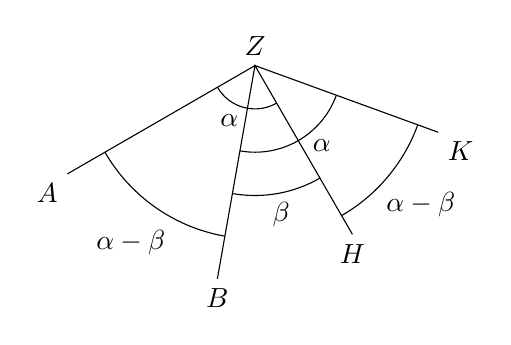
\begin{tikzpicture}[scale=.55]
\coordinate (Z) at (0,0);
\coordinate (A) at (-150:5cm);
\coordinate (B) at (-100:5cm);
\coordinate (H) at (-60:4.5cm);
\coordinate (K) at (-20:4.5cm);
\draw (A) node[below left] {$A$} -- (Z) node[above] {$Z$} -- (B) node[below] {$B$};
\draw (H) node[below] {$H$} -- (Z) -- (K) node[below right] {$K$};
\draw (-150:1cm) arc (-150:-60:1);
\draw (-100:2cm) arc (-100:-20:2);
\draw (-100:3cm) arc (-100:-60:3);
\draw (-150:4cm) arc (-150:-100:4);
\draw (-60:4cm) arc (-60:-20:4);
\node at (-115:1.4) {$\alpha$};
\node at (-50:2.4) {$\alpha$};
\node at (-80:3.5) {$\beta$};
\node at (-40:5) {$\alpha - \beta$};
\node at (-125:5) {$\alpha - \beta$};
\end{tikzpicture}
\caption{$\angle AZB=\angle HZK$}\label{f.compass-relative4}
\end{subfigure}
\end{center}
\end{figure}

%\begin{center}
%
%\begin{tikzpicture}[scale=.45]
%\coordinate (Z) at (0,0);
%\coordinate (A) at (-130:5cm);
%\coordinate (B) at (-90:5cm);
%\fill (Z) node[above left] {$Z$} circle[radius=3pt];
%\fill (A) node[below left] {$A$} circle[radius=3pt];
%\fill (B) node[below] {$B$} circle[radius=3pt];
%\draw[name path=c1] (Z) circle[radius=5cm];
%\draw[name path=c2] (Z) circle[radius=2.5cm];
%\node at (2,5) {$c_1$};
%\node at (2,2.5) {$c_2$};
%\draw[thick,dashed] (A) -- node[below,yshift=-6pt] {$s$} (B);
%\draw[thick] (A) -- node[above] {$w$} +(20:120pt) coordinate (H);
%\fill (H) node[above right,xshift=-5pt,yshift=3pt] {$H$} circle[radius=3pt];
%\draw[thick] (B) -- node[right] {$w$} +(60:120pt) coordinate (K);
%\fill (K) node[right] {$K$} circle[radius=3pt];
%\draw[thick] (Z) -- node[left,xshift=-2pt,yshift=-2pt] {$m$} (A);
%\draw[thick] (Z) -- (B);
%\draw[thick] (Z) -- (H);
%\draw[thick] (Z) -- node[above] {$n$} (K);
%\draw[thick,dashed] (H) -- (K);
%\end{tikzpicture}
%\end{center}

מ-%
$\triangle AZH \cong \triangle BZK$
נובע
$\angle AZB = \angle HZK$.
קשה לראות את השוויונות הללו באיור, אבל האיור שלהלן מבהיר את היחסים בין הזוויות. נגדיר
$\alpha = \angle AZH = \angle BZK$
ו-%
$\beta = \angle BZH$,
וקל לראות ש-%
$\angle AZB = \angle HZK = \alpha - \beta$
(\ref{f.compass-relative4}).

%\begin{center}
%
%\begin{tikzpicture}[scale=.6]
%\coordinate (Z) at (0,0);
%\coordinate (A) at (-150:5cm);
%\coordinate (B) at (-100:5cm);
%\coordinate (H) at (-60:4.5cm);
%\coordinate (K) at (-20:4.5cm);
%\fill (Z) circle[radius=2pt];
%\fill (A) circle[radius=2pt];
%\fill (B) circle[radius=2pt];
%\fill (H) circle[radius=2pt];
%\fill (K) circle[radius=2pt];
%\draw[thick] (A) node[below left] {$A$} -- (Z) node[above] {$Z$} -- (B) node[below] {$B$};
%\draw[thick] (H) node[below] {$H$} -- (Z) -- (K) node[below right] {$K$};
%\draw (-150:1cm) arc (-150:-60:1);
%\draw (-100:2cm) arc (-100:-20:2);
%\draw (-100:3cm) arc (-100:-60:3);
%\draw[thick,dashed] (-150:4cm) arc (-150:-100:4);
%\draw[thick,dashed] (-60:4cm) arc (-60:-20:4);
%\node at (-115:1.4) {$\alpha$};
%\node at (-50:2.4) {$\alpha$};
%\node at (-80:3.5) {$\beta$};
%\node at (-40:5) {$\alpha - \beta$};
%\node at (-125:5) {$\alpha - \beta$};
%\end{tikzpicture}
%\end{center}
%$\triangle AZB\sim\triangle HZK$
%כי הראנו ששני המשולשים הם שווי-שוקיים עם זוויות קודקוד שוות.
%\begin{center}
%
%\begin{tikzpicture}[scale=.45]
%\coordinate (Z) at (0,0);
%\coordinate (A) at (-130:5cm);
%\coordinate (B) at (-90:5cm);
%\fill (Z) node[above left] {$Z$} circle[radius=4pt];
%\fill (A) node[below left] {$A$} circle[radius=3pt];
%\fill (B) node[below] {$B$} circle[radius=3pt];
%\draw[name path=c1] (Z) circle[radius=5cm];
%\draw[name path=c2] (Z) circle[radius=2.5cm];
%\node at (2,5) {$c_1$};
%\node at (2,2.5) {$c_2$};
%\draw[thick] (A) -- node[below,yshift=-6pt] {$s$} (B);
%\path[thick,dashed] (A) -- +(20:120pt) coordinate (H);
%\fill (H) node[below] {$H$} circle[radius=3pt];
%\path[thick,dashed] (B) -- +(60:120pt) coordinate (K);
%\fill (K) node[right] {$K$} circle[radius=3pt];
%\draw[thick] (Z) -- node[left,xshift=-2pt,yshift=-2pt] {$m$} (A);
%\draw[thick] (Z) -- (B);
%\draw[thick] (Z) -- (H);
%\draw[thick] (Z) -- node[above] {$n$} (K);
%\draw[thick] (H) -- node[below right] {$x$} (K);
%\draw[thick,dashed] (A) -- (H);
%\draw[thick,dashed] (B) -- (K);
%\end{tikzpicture}
%\end{center}

סמנו את קטע הקו
$\overline{HK}$
ב-%
$x$,
ונקבל:

\begin{eqn}
\frac{m}{s} &=& \frac{n}{x}\\
x&=&\frac{n}{m}s\,.
\end{eqn}
\end{proof}

%%%%%%%%%%%%%%%%%%%%%%%%%%%%%%%%%%%%%%%%%%%%%%%%%%%%%%%%%%%%%%%

\section{מציאת נקודת החיתוך של שני קווים}
\label{s.two-lines}

\begin{theorem}
נתונים שני קווים המכילים את קטעי הקו
$\overline{AB},\overline{CD}$.
ניתן לבנות את נקודת החיתוך שלהם.
\end{theorem}
\begin{proof}
בנו את
$C'$,
השיקוף של
$C$
מסביב ל-%
$\overline{AB}$,
ו-%
$D'$
השיקוף של
$D$
מסביב ל-%
$\overline{AB}$.
יש שני מקרים תלוי אם 
$C,D$ 
נמצאים בשני הצדדים של
$\overline{AB}$
או באותו צד כפי שניתן לראות באיורים%
~\ref{f.compass-intersection1}, \ref{f.compass-intersection2}.

\textbf{מקרה $1$:}
נקודת החיתוך
$S$
נמצאת על הקו
$\overline{AB}$
כי
$\triangle CZS\cong \triangle C'ZS$
לפי צלע-זווית-צלע:
$\overline{CZ}=\overline{C'Z}$,
$\angle CZS = \angle C'ZS = 90^\circ$
ו-%
$\overline{ZS}$
צלע משותף. מכאן ש-%
$\overline{C'S}=\overline{CS}$,
ובאופן דומה
$\overline{D'S}=\overline{DS}$.

\begin{figure}[htb]
\begin{center}
\begin{tikzpicture}[scale=.9]
\coordinate (A) at (-4,0);
\coordinate (B) at (2,0);
\coordinate (C) at (-3,2);
\coordinate (D) at (1,-1);
\coordinate (Cp) at (-3,-2);
\coordinate (Dp) at (1,1);
\vertex{A};
\vertex{B};
\node[below] at (A) {$A$};
\node[below] at (B) {$B$};
\node[above] at (C) {$C$};
\node[below] at (D) {$D$};
\node[below] at (Cp) {$C'$};
\node[above] at (Dp) {$D'$};
\draw[name path=ab] ($(A)!1.3!(B)$) -- ($(B)!1.3!(A)$);
\draw[name path=cd] ($(C)!1.2!(D)$) -- ($(D)!1.1!(C)$);
\path [name intersections={of=ab and cd,by={S}}];
\node[above] at (S) {$S$};
\draw (Cp) -- node[below] {$x$} (S);
\draw (S) -- node[above,xshift=-5pt] {$e\!-\!x$} (Dp);
\draw (C) -- node[above left,yshift=6pt] {$c$} (Cp);
\draw (D) -- node[above right,yshift=6pt] {$d$} (Dp);
\path (C) -- node[right,xshift=2pt] {$x$} (S);
\path (S) -- node[left,near end,xshift=-2pt] {$e\!-\!x$} (D);
\node[below left] at (C|-A) {$Z$};
\vertex{C};
\vertex{D};
\vertex{Cp};
\vertex{Dp};
\draw ($(C)!.5!(Cp)$) rectangle +(6pt,6pt);
\draw[rotate=90] ($(D)!.5!(Dp)$) rectangle +(6pt,6pt);
\end{tikzpicture}
\end{center}
\caption{בניית החיתוך של שני קווים (1)}\label{f.compass-intersection1}
\end{figure}

%\begin{center}
%\begin{tikzpicture}[scale=.8]
%\coordinate (A) at (-4,0);
%\coordinate (B) at (2,0);
%\coordinate (C) at (-3,2);
%\coordinate (D) at (1,-1);
%\coordinate (Cp) at (-3,-2);
%\coordinate (Dp) at (1,1);
%\fill (A) node[below] {$A$} circle[radius=1.5pt];
%\fill (B) node[below] {$B$} circle[radius=1.5pt];
%\fill (C) node[above] {$C$} circle[radius=1.5pt];
%\fill (D) node[below] {$D$} circle[radius=1.5pt];
%\fill (Cp) node[below] {$C'$} circle[radius=1.5pt];
%\fill (Dp) node[above] {$D'$} circle[radius=1.5pt];
%\draw[name path=ab] ($(A)!1.3!(B)$) -- ($(B)!1.3!(A)$);
%\draw[name path=cd] ($(C)!1.2!(D)$) -- ($(D)!1.1!(C)$);
%\path [name intersections={of=ab and cd,by={S}}];
%\fill (S) node[above] {$S$} circle[radius=1.5pt];
%\draw (Cp) -- (Dp);
%\draw[thick,dashed] (C) -- node[above left] {$c$} (Cp);
%\draw[thick,dashed] (D) -- node[above right] {$d$} (Dp);
%\path (C) -- node[right,xshift=1.5pt] {$x$} (S);
%\path (S) -- node[left,near end,xshift=-2pt] {$e-x$} (D);
%\node at (1,-2.5) {\mbox{\boldmath $\overline{CD}=\overline{C'D'}=e$}};
%\coordinate (Z) at (-3,0);
%\fill (Z) node[below right] {$Z$} circle[radius=1.5pt];
%\draw (Z) rectangle +(8pt,8pt);
%\end{tikzpicture}
%\end{center}

סמנו
$x = \overline{CS}, c = \overline{CC'}, d = \overline{DD'}, e = \overline{CD}$.
$\triangle CSC'\sim\triangle DSD'$
ולכן
$\disfrac{x}{e-x} = \disfrac{c}{d}$.
נפתור את המשוואה עבור
$x$
ונקבל
$x=\disfrac{c}{c+d}e$.

\textbf{מקרה $2$:}
$\triangle CSC'\sim\triangle DSD'$,
ולכן
$\disfrac{x}{x-e}=\disfrac{c}{d}$
ו-%
$x=\disfrac{c}{c-d}e$.

\begin{figure}[htb]
\begin{center}
\begin{tikzpicture}[scale=.9]
\coordinate (A) at (-4,0);
\coordinate (B) at (2,0);
\coordinate (C) at (-3,2);
\coordinate (D) at (-1,1);
\coordinate (Cp) at (-3,-2);
\coordinate (Dp) at (-1,-1);
\vertex{A};
\vertex{B};
\node[below] at (A) {$A$};
\node[below] at (B) {$B$};
\node[above] at (C) {$C$};
\node[above] at (D) {$D$};
\node[below] at (Cp) {$C'$};
\node[below] at (Dp) {$D'$};
\draw[name path=ab] ($(A)!1.3!(B)$) -- ($(B)!1.3!(A)$);
\draw[name path=cd] ($(C)!2.2!(D)$) -- ($(D)!1.1!(C)$);
\path [name intersections={of=ab and cd,by={S}}];
\node[above] at (S) {$S$};
\draw (Cp) -- (S);
\draw (C) -- node[above left,yshift=6pt] {$c$} (Cp);
\draw (D) -- node[above right,yshift=6pt] {$d$} (Dp);
\path (C) -- node[above] {$e$} (D);
\path (Cp) -- node[below] {$e$} (Dp);
\path (D) -- node[above right,xshift=-4pt] {$x-e$} (S);
\path (Dp) -- node[below right,xshift=-4pt] {$x-e$} (S);
\node[below left] at (C|-A) {$Z$};
\vertex{C};
\vertex{D};
\vertex{Cp};
\vertex{Dp};
\draw ($(C)!.5!(Cp)$) rectangle +(6pt,6pt);
\draw[rotate=90] ($(D)!.5!(Dp)$) rectangle +(6pt,6pt);
\end{tikzpicture}
\end{center}
\caption{בניית החיתוך של שני קווים (2)}\label{f.compass-intersection2}
\end{figure}



בנו את המעגלים
$c(C',d)$
,
$c(D,e)$
וסמנו את נקודת החיתוך שלהם ב-%
$H$
(איור%
~\ref{f.compass-intersection3}).

סכום האורכים של
$\overline{CC'},\overline{C'H}$
הוא
$c + d$.
אם
$H$
נמצאת בהמשך הקו של
$\overline{CC'}$,
אז האורך של
$\overline{CH}$
הוא
$c+d$.
במקרה ש-%
$C,D$
נמצאות על אותו צד של
$\overline{AB}$, 
$\overline{CH} = c - d$.

\begin{figure}[htb]
\begin{center}
\begin{tikzpicture}[scale=.8]
\coordinate (A) at (-4,0);
\coordinate (B) at (2,0);
\coordinate (C) at (-3,2);
\coordinate (D) at (1,-1);
\coordinate (Cp) at (-3,-2);
\coordinate (Dp) at (1,1);
\vertex{A};
\vertex{B};
\node[below left] at (A) {$A$};
\node[below] at (B) {$B$};
\node[above] at (C) {$C$};
\node[below] at (D) {$D$};
\node[left] at (Cp) {$C'$};
\node[above] at (Dp) {$D'$};
\draw[name path=ab] ($(A)!1.3!(B)$) -- ($(B)!1.3!(A)$);
\draw[name path=cd] ($(C)!1.2!(D)$) -- ($(D)!1.1!(C)$);
\path [name intersections={of=ab and cd,by={S}}];
\node[above,yshift=4pt] at (S) {$S$};
\draw (Cp) -- node[below right,xshift=5pt,yshift=5pt] {$e$} (Dp);
\path (C) -- node[above left] {$c$} (Cp);
\draw[thick,dashed] (D) -- node[above right] {$d$} (Dp);
\draw[name path=circled] (D) let
  \p1 = ($ (D) - (C) $),
  \n2 = {veclen(\x1,\y1)}
in
  ++(130:\n2) arc (130:230:\n2);

\draw[name path=circlecp] (Cp) let
  \p1 = ($ (D) - (Dp) $),
  \n2 = {veclen(\x1,\y1)}
in
  ++(-180:\n2) arc (-180:0:\n2);
\path [name intersections={of=circled and circlecp,by={H}}];
\node[below left] at (H) {$H$};
\draw ($(C)!1.2!(H)$) -- (C);
\draw (H) -- node[right] {$d$} (Cp);
\draw (D) -- node[right,xshift=18pt,yshift=12pt] {$e$} (H);
\vertex{Cp};
\vertex{D};
\vertex{C};
\vertex{Dp};
\vertex{H};
\path (C) -- node[above] {$x$} (S);
\path (Cp) -- node[below] {$x$} (S);
\end{tikzpicture}
\end{center}
\caption{בניית החיתוך של שני קווים (3)}\label{f.compass-intersection3}
\end{figure}


$H$
היא החיתוך של 
$c(C',d),c(D,e)$,
ולכן
$\overline{C'H}=d,\overline{DH}=e$,
אבל 
$\overline{C'D'}=e, \overline{DD'}=e$,
ולכן המרובע
$C'D'DH$
הוא מקבילית. לפי הבניה, קטע הקו
$\overline{DD'}$
מקביל ל-%
$\overline{CC'}$,
ולכן
$\overline{C'H}$,
שמקביל ל-%
$\overline{DD'}$
במקבילית, מקביל גם ל-%
$\overline{CC'}$.

\begin{figure}[htb]
\begin{center}
\begin{tikzpicture}[scale=.9]
\coordinate (A) at (-4,0);
\coordinate (B) at (2,0);
\coordinate (C) at (-3,2);
\coordinate (D) at (1,-1);
\coordinate (Cp) at (-3,-2);
\coordinate (Dp) at (1,1);
\vertex{A};
\vertex{B};
\node[below left] at (A) {$A$};
\node[below] at (B) {$B$};
\node[above] at (C) {$C$};
\node[below] at (D) {$D$};
\node[left] at (Cp) {$C'$};
\node[above] at (Dp) {$D'$};
\draw[name path=ab] ($(A)!1.3!(B)$) -- ($(B)!1.3!(A)$);
\draw[name path=cd] ($(C)!1.2!(D)$) -- ($(D)!1.1!(C)$);
\path [name intersections={of=ab and cd,by={S}}];
\node[above,yshift=4pt] at (S) {$S$};
\draw (Cp) -- (Dp);
\path (C) -- node[above,yshift=4pt] {$x$} (S);
\path (Cp) -- node[below,yshift=-4pt] {$x$} (S);
\path (C) -- node[above left] {$c$} (Cp);
\draw (D) -- node[above right] {$d$} (Dp);
\draw[name path=circled] (C) let
  \p1 = ($ (S) - (C) $),
  \n2 = {veclen(\x1,\y1)}
in
  ++(-10:\n2) arc (-10:-100:\n2);

\draw[name path=circlecp] (Cp) let
  \p1 = ($ (S) - (C) $),
  \n2 = {veclen(\x1,\y1)}
in
  ++(100:\n2) arc (100:0:\n2);
\draw (Cp) -- (C);
\vertex{C};
\vertex{Cp};
\vertex{D};
\vertex{Dp};
\end{tikzpicture}
\end{center}
\caption{בניית החיתוך של שני קווים (4)}\label{f.compass-intersection4}
\end{figure}


%\begin{center}
%\begin{tikzpicture}[scale=.8]
%\coordinate (A) at (-4,0);
%\coordinate (B) at (2,0);
%\coordinate (C) at (-3,2);
%\coordinate (D) at (1,-1);
%\coordinate (Cp) at (-3,-2);
%\coordinate (Dp) at (1,1);
%\fill (A) node[below left] {$A$} circle[radius=1.5pt];
%\fill (B) node[below] {$B$} circle[radius=1.5pt];
%\fill (C) node[above] {$C$} circle[radius=1.5pt];
%\fill (D) node[below] {$D$} circle[radius=1.5pt];
%\fill (Cp) node[left] {$C'$} circle[radius=1.5pt];
%\fill (Dp) node[above] {$D'$} circle[radius=1.5pt];
%\draw[name path=ab] ($(A)!1.3!(B)$) -- ($(B)!1.3!(A)$);
%\draw[name path=cd] ($(C)!1.2!(D)$) -- ($(D)!1.1!(C)$);
%\path [name intersections={of=ab and cd,by={S}}];
%\fill (S) node[above,yshift=4pt] {$S$} circle[radius=1.5pt];
%\draw (Cp) -- (Dp);
%\path (C) -- node[above,yshift=4pt] {$x$} (S);
%\path (Cp) -- node[below,yshift=-4pt] {$x$} (S);
%\path (C) -- node[above left] {$c$} (Cp);
%\draw[thick,dashed] (D) -- node[above right] {$d$} (Dp);
%\node at (3,-3) {\mbox{\boldmath $\overline{CD}=\overline{C'D'}=\overline{DH}=e$}};
%\draw[name path=circled] (C) let
%  \p1 = ($ (S) - (C) $),
%  \n2 = {veclen(\x1,\y1)}
%in
%  ++(-10:\n2) arc (-10:-100:\n2);
%
%\draw[name path=circlecp] (Cp) let
%  \p1 = ($ (S) - (C) $),
%  \n2 = {veclen(\x1,\y1)}
%in
%  ++(100:\n2) arc (100:0:\n2);
%\draw[thick,dashed] (Cp) -- (C);
%\end{tikzpicture}
%\end{center}




אחת מנקודות הקצה של הקטע היא
$C'$
והקטע חייב להיות על ההמשך של הקטע
$\overline{CC'}$.
האורכים
$c,d,e$
נתונים ולפי משפט
~\ref{thm.add-subtract-mm}
ניתן לבנות קטע באורך
$c+d$,
ולפי משפט
\ref{thm.ratio}
ניתן לבנות קטע באורך
$x=\disfrac{c}{c+d}e$.
$S$
היא נקודת החיתוך של המעגלים
$c(C,x)$
ו-%
$c(C',x)$
(איור%
~\ref{f.compass-intersection4}).
\end{proof}

\section{מציאת נקודת החיתוך של קו עם מעגל}\label{s.line-circle}

\begin{theorem}
נתון מעגל
$k=C(M,r)$
וקו
$\overline{AB}$.
ניתן לבנות את נקודות החיתוך שלהם.
\end{theorem}


%%%%%%%%%%%%%%%%%%%%%%%%%%%%%%%%%%%%%%%%%%%%%%%%%%%%%%%%%%%%%%%

בנו את 
$M'$,
השיקוף של
$M$
מסביב ל-%
$\overline{AB}$,
והמעגל
$k'=c(M',r)$.
נקודות החיתוך של המעגלים
$k,k'$
הן נקודות החיתוך של הקו 
$\overline{AB}$
והמעגל
$k$
(איור%
~\ref{f.compass-circle4}).

\begin{figure}[htb]
\begin{center}
\begin{tikzpicture}[scale=.5]
\coordinate (A) at (-7,0);
\coordinate (B) at (8,0);
\coordinate (M) at (0,-2);
\coordinate (Mp) at (0,2);
\node[below left] at (M) {$M$};
\node[above left] at (Mp) {$M'$};
\draw[name path=c1] (M) circle[radius=3cm];
\draw[name path=c2] (Mp) circle[radius=3cm];
\draw[name path=ab] ($(A)!1.2!(B)$) --
  node[above,very near end] {$l$} ($(B)!1.2!(A)$);
\path [name intersections={of=c1 and c2,by={S1,S2}}];
\path[name path=radius1] (M) -- ++(15:4cm);
\path [name intersections={of=c1 and radius1,by={R1}}];
\draw (M) -- node[below] {$r$} (R1);
\path[name path=radius2] (Mp) -- ++(40:4cm);
\path [name intersections={of=c2 and radius2,by={R2}}];
\draw (Mp) -- node[above] {$r$} (R2);
\draw (Mp) -- (M) -- (S1) -- (Mp) -- (S2) -- (M);
\node[right,xshift=6pt,yshift=6pt] at (S1) {$X$};
\node[left,xshift=-6pt,yshift=6pt] at (S2) {$Y$};
\draw (0,0) rectangle +(10pt,10pt);
\node at (-3.5,-3) {$k$};
\node at (-3.5,3) {$k'$};
\end{tikzpicture}
\end{center}
\caption{בניית החיתוך של קו מעגל (1)}\label{f.compass-circle4}
\end{figure}


בניה זו אינה אפשרית אם מרכז המעגל
$M$
נמצא על הקו
$\overline{AB}$.
במקרה זה, יש להאריך ולקצר את הקטע
$\overline{AM}$
באורך 
$r$
לפי משפט~%
~\ref{thm.add-subtract-mm}.
נקודות הקצה של הקטעים הללו הן נקודות החיתוך של
$k$
עם
$\overline{AB}$
(איור%
~\ref{f.compass-circle5}).

\begin{figure}[htb]
\begin{center}
\begin{tikzpicture}[scale=.5]
\coordinate (A) at (-7,0);
\coordinate (B) at (8,0);
\coordinate (M) at (0,0);
\vertex{M};
\vertex{A};
\node[below] at (A) {$A$};
\node[below left] at (M) {$M$};
\draw[name path=c1] (M) circle[radius=3cm];
\draw[name path=ab] ($(A)!1.2!(B)$) -- 
  node[above,very near end] {$l$} ($(B)!1.2!(A)$);
\path[name path=radius1] (M) -- ++(50:4cm);
\path [name intersections={of=c1 and radius1,by={R1}}];
\draw (M) -- node[above] {$r$} (R1);
\path [name intersections={of=c1 and ab,by={S1,S2}}];
\node[above right] at (S1) {$X$};
\node[above left] at (S2) {$Y$};
\path (M) -- node[below,xshift=4pt] {$\overline{AM}+r$} (S1);
\path (A) -- node[below] {$\overline{AM}-r$} (S2);
\node at (-2.5,2.5) {$k$};
\end{tikzpicture}
\end{center}
\caption{בניית החיתוך של קו מעגל (2)}\label{f.compass-circle5}
\end{figure}


%\begin{center}
%\begin{tikzpicture}[scale=.4]
%\coordinate (A) at (-7,0);
%\coordinate (B) at (8,0);
%\coordinate (M) at (0,0);
%\fill (A) node[below] {$A$} circle[radius=3pt];
%\fill (B) node[below] {$B$} circle[radius=3pt];
%\fill (M) node[below left] {$M$} circle[radius=3pt];
%\draw[name path=c1] (M) circle[radius=3cm];
%\draw[name path=ab] ($(A)!1.2!(B)$) -- ($(B)!1.2!(A)$);
%\path[name path=radius1] (M) -- ++(-30:4cm);
%\path [name intersections={of=c1 and radius1,by={R1}}];
%\draw[thick,dashed] (M) -- node[below] {$r$} (R1);
%\path [name intersections={of=c1 and ab,by={S1,S2}}];
%\fill (S1) node[above right] {$AM+r$} circle[radius=3pt];
%\fill (S2) node[above left] {$AM-r$} circle[radius=3pt];
%\fill (R1) circle[radius=3pt];
%\end{tikzpicture}
%\end{center}

%%%%%%%%%%%%%%%%%%%%%%%%%%%%%%%%%%%%%%%%%%%%%%%%%%%%%%%%%%%%%%%

\subsection*{מהי ההפתעה?}

כאשר לומדים על בניות עם סרגל ומחוגה, ברור מאליו ששני הכלים נחוצים, ולכן מפתיע מאוד לגלות שמחוגה בלבד מספיקה. ההוכחה די ארוכה כך שלא נשאיר את הסרגל בבית, אבל המשפט מראה שאין להניח שאין חלופות למושגים מתמטיים ידועים.

%%%%%%%%%%%%%%%%%%%%%%%%%%%%%%%%%%%%%%%%%%%%%%%%%%%%%%%%%%%%%%%

\subsection*{מקודות}

בפרק זה מבוסס על בעיה מספר
$33$
ב-%
\L{\cite{dorrie1}}
ועל העיבוד שלה על ידי
\L{Michael Woltermann} \L{\cite{dorrie2}}.
הוכחה נוספת ניתן למוצא ב-%
\L{\cite{mm}}.
